\documentclass[UTF8, a4paper, zihao=-4, bibliography=totoc]{ctexart}
\usepackage{color}
\usepackage[dvipsnames]{xcolor}
\usepackage{mathtools}
\usepackage[colorlinks=true, pdfstartview=FitH, linkcolor=black, anchorcolor=violet, citecolor=magenta]{hyperref}
\usepackage{graphicx}
\usepackage{enumitem}
\usepackage{titlesec}
\usepackage{titletoc}
\usepackage{bm}
\usepackage{amsmath}
\usepackage{amsfonts}
\usepackage{mathrsfs}
\usepackage{multirow}
\usepackage{amsthm}
\usepackage{tabularx, booktabs}
\usepackage{longtable}
\usepackage{supertabular}
\usepackage{array, makecell}
\usepackage{graphicx}
\usepackage{epstopdf}
\usepackage{float}
\usepackage{subfigure}
\usepackage{geometry}
\usepackage{ctex}
\usepackage{listings}
\usepackage[nottoc,numbib]{tocbibind}
\usepackage[backend=biber, style=gb7714-2015]{biblatex}
\addbibresource[location=local]{../reference.bib}
\usepackage{pythonhighlight}
\usepackage{caption}
\usepackage{booktabs}
\usepackage{algorithm}
\usepackage{algorithmic}
\usepackage[toc]{appendix}
\usepackage{xhfill}
%%%%%%%%%%%%%%%%%%%%%%%%%%%%%%%%%%%%%%%%%%%%%%%%%%%%%%%%%%%%%%%%%%%%%%%%%%%%%%%%
%%%%%%%%%%%%%%%%%%%%%%%%%%%%%%%%% ctexset %%%%%%%%%%%%%%%%%%%%%%%%%%%%%%%%%%%%%%
%%%%%%%%%%%%%%%%%%%%%%%%%%%%%%%%%%%%%%%%%%%%%%%%%%%%%%%%%%%%%%%%%%%%%%%%%%%%%%%%
\ctexset{
    bibname     =   {参考文献},
    section = {
        number  =   \arabic{section},
        format  +=  \zihao{-4}\raggedright,
        name    =   {,.},
    },
    subsection = {
        format  =  \bf{\zihao{-4}}\raggedright,
    },
    subsubsection = {
        number  =   \arabic{subsubsection},
        format  +=  {\zihao{-4}}\raggedright,
    }
}

% 用来设置附录中代码的样式

\definecolor{mygreen}{RGB}{28,172,0} % color values Red, Green, Blue
\definecolor{mylilas}{RGB}{170,55,241}

\lstset{
    basicstyle          =   \sffamily,
    keywordstyle        =   \bfseries,
    commentstyle        =   \rmfamily\itshape,
    stringstyle         =   \ttfamily,
    flexiblecolumns,
    numbers             =   left,
    showspaces          =   false,
    numberstyle         =   \zihao{-5}\ttfamily,
    showstringspaces    =   false,
    captionpos          =   t,
    frame               =   lrtb,
}

\lstdefinestyle{Python}{
    language        =   Python,
    basicstyle      =   \zihao{-5}\ttfamily,
    numberstyle     =   \zihao{-5}\ttfamily,
    keywordstyle    =   \color{blue},
    keywordstyle    =   [2] \color{teal}, % just to check that it works
    stringstyle     =   \color{magenta},
    commentstyle    =   \color{mygreen}\ttfamily,
    breaklines      =   true,
    columns         =   fixed,
    basewidth       =   0.5em,
}

\lstdefinestyle{MATLAB}{
    language        =   Matlab,
    basicstyle      =   \zihao{-5}\ttfamily,
    numberstyle     =   \zihao{-5}\ttfamily,
    keywordstyle    =   \color{blue},
    keywordstyle    =   [2] \color{teal}, % just to check that it works
    stringstyle     =   \color{mylilas},
    commentstyle    =   \color{mygreen}\ttfamily,
    breaklines      =   true,
    columns         =   fixed,
    basewidth       =   0.5em,
}

\theoremstyle{definition}

\newtheorem{definition}{定义}[section]

\newtheorem{theorem}{定理}[section]

\newtheorem{corollary}{推论}[theorem]

\newtheorem{lemma}[theorem]{引理}

\newenvironment{myquote}
    {\begin{quote}\kaishu\zihao{5}}
    {\end{quote}}

\setcounter{MaxMatrixCols}{20}

\renewcommand{\algorithmicrequire}{ \textbf{Input:}} %Use Input in the format of Algorithm 
\renewcommand{\algorithmicensure}{ \textbf{Output:}} %UseOutput in the format of Algorithm
% 定义页面边距

\newgeometry{
    left=2.5cm,
    right=2.0cm,
    top=2.5cm,
    bottom=2.5cm
}

\newcommand{\ThisProjectTitle}{解线性方程组的迭代法}
\newcommand{\ThisDate}{2017-11-28}
\newcommand{\ThisNo}{No.2}

%%%%%%%%%%%%%%%%%%%%%%%%%%%%%%%%%%%%%%%%%%%%%%%%%%%%%%%%%%%%%%%%%%%%%%%%%%%%%%%%
%%%%%%%%%%%%%%%%%%%%%%%%%%%%%%%%%%% document %%%%%%%%%%%%%%%%%%%%%%%%%%%%%%%%%%%
%%%%%%%%%%%%%%%%%%%%%%%%%%%%%%%%%%%%%%%%%%%%%%%%%%%%%%%%%%%%%%%%%%%%%%%%%%%%%%%%

\begin{document}

\newcommand{\CourseName}{{\bf 课程名称:}}
\newcommand{\Grade}{{\bf 年级:}}
\newcommand{\Score}{{\bf 上机实践成绩:}}
\newcommand{\Director}{{\bf 指导教师:}}
\newcommand{\StudentName}{{\bf 学生姓名:}}
\newcommand{\ProjectTitle}{{\bf 上机实践名称:}}
\newcommand{\StudentID}{{\bf 学号:}}
\newcommand{\Date}{{\bf 上机实践日期:}}
\newcommand{\No}{{\bf 上机实践编号:}}
\newcommand{\GroupNum}{{\bf 组号:}}
\newcommand{\LastEditTine}{{\bf 最后修改时间:}}

\newcommand{\ThisCourseName}{数值计算实验}
\newcommand{\MyGrade}{2015级}
\newcommand{\MyScore}{100}
\newcommand{\MyDirector}{朱娟萍}
\newcommand{\MyName}{刘鹏}
\newcommand{\ThisProjectTitle}{非线性方程求根}
\newcommand{\MyID}{20151910042}
\newcommand{\ThisDate}{2017-10-16}
\newcommand{\ThisNo}{No.1}
\newcommand{\MyGroupNum}{1}
\newcommand{\MyLastEditTine}{\today}

\newcommand{\HRule}{\rule{\linewidth}{0.3mm}}
\newcommand{\xfill}[2][1ex]{{%
  \dimen0=#2\advance\dimen0 by #1
  \leaders\hrule height \dimen0 depth -#1\hfill%
}}
\newcommand{\xfilll}[2][1ex]{%
  \dimen0=#2\advance\dimen0 by #1%
  \leaders\hrule height \dimen0 depth -#1\hfill%
}

\begin{center}
    {\zihao{3} \bf 云南大学数学与统计学院}\\
    {\zihao{3} \bf 上机实践报告}
\end{center}

\begin{table}[h]
    \centering
    \resizebox{\textwidth}{!}{%
        \begin{tabular}{|l|l|l|}
        \hline
            \CourseName \ThisCourseName     & \Grade \MyGrade       & \Score                        \\ \hline
            \Director \MyDirector           & \StudentName \MyName  &                               \\ \hline
            \ProjectTitle \ThisProjectTitle & \StudentID \MyID      & \Date \ThisDate               \\ \hline
            \No \ThisNo                     & \GroupNum             & \LastEditTine \MyLastEditTine \\ \hline
        \end{tabular}
    }
    \xfill{30pt}
\end{table}

\section{实验目的}

1. 通过对所学的线性方程组直接求解的理论方法进行编程,提升程序编写水平;

2. 通过对理论方法的编程实验,进一步掌握理论方法的每一个细节;

3. 通过数值法求解,发现数值方法与符号方法的区别,并形成专业思维。

\section{实验内容}

1. 编程实现高斯-若尔当列主元消元法;

2. 编程实现高斯-若尔当全主元消元法;

3. 任选一种方案,Doolittle分解或者Crout分解,编程实现矩阵的LU分解;

4. 编程实现三对角线矩阵的稀疏方式存储,然后对其进行LU分解。

\section{实验平台}

macOS

Python 3.7.3;

MATLAB R2017b win64;

\section{实验记录与实验结果分析}

\subsection{第1题}

1题
编程实现:用高斯-若尔当列主元消元法求下列方程的解[1]:

\begin{equation}
    \left\{\begin{aligned}
        x_{1}+2 x_{2}+x_{3}     &=  2   \\
        -2 x_{1}-2 x_{2}-x_{3}  &=  -3  \\
        2 x_{1}-3 x_{2}-2 x_{3} &=  -1 
    \end{aligned}\right.
\end{equation}

\subsubsection{程序代码}

\lstinputlisting[
    style       =   Python,
    %caption     =   {\bf ff.py},
    label       =   {get_root.py}
]{../../src/3_线性方程组的直接解法/ColumnPivotMethod.py}

\subsubsection{运行结果}

\subsubsection{结果分析}

由于二分法与埃特金方法的函数并不是一样的,前者是原函数,后者是迭代函数,所以很难写一个通用算法解决这个迭代函数的生成问题。所以这个class意义不是很大,不过可以通过对属性进行赋值,重复进行计算,也算有一定的灵活性。

\section{实验体会}

通过编程,复习了简单迭代法及其改进。明白了二分法与埃特金法的斯坦弗森过程之间的区别。

\section{参考文献}

[1] 金一庆, 陈越, 王冬梅. 数值方法[M]. 北京: 机械工业出版社; 2000.2.


\section{实验目的}
\begin{enumerate}[leftmargin=1.4cm, itemsep=-0.5mm]
    \item 通过对所学的线性方程组迭代求解的理论方法进行编程,提升程序编写水平;
    \item 通过对理论方法的编程实验,进一步掌握理论方法的每一个细节;
    \item 通过数值法求解,掌握判断循环终结的条件,理解矩阵范数的存在意义。
    
\end{enumerate}

\section{实验内容}
\begin{enumerate}[leftmargin=1.4cm, itemsep=-0.5mm]
    \item 编制求矩阵的各种范数的程序;
    \item 编程实现用雅可比迭代法求线性方程组的数值解;
    \item 编程实现用高斯-塞德尔方法求线性方程组的数值解;
    \item 编程实现用SOR方法求线性方程组的数值解。
\end{enumerate}

\section{实验平台}

macOS

Python 3.7.3

MATLAB R2019a

\section{实验记录与实验结果分析}

\subsection{第1题}
\begin{quote}
    {\kaishu
    对下列矩阵计算$\|\cdot\|_{\infty}$,$\|\cdot\|_{1}$,$\|\cdot\|_{2}$:
    (1)\begin{equation}
            \mathbf{A}=\left[ \begin{array}{rr}{1} & {-1} \\ {2} & {1}\end{array}\right]
        \end{equation}
    (2) \begin{equation}
            \mathbf{B}=\left[ \begin{array}{rr}{10} & {15} \\ {0} & {1}\end{array}\right]
        \end{equation}
    (3) \begin{equation}
            \mathbf{C}=\left[ \begin{array}{rr}{0.6} & {-0.5} \\ {-0.1} & {0.3}\end{array}\right]
        \end{equation}
    }
\end{quote}

在一般的无大型模块导入的情况下,对于行范数与列范数而言,求解都是比较简单的,但是对于谱范数却并不是很容易,首先一点,难以做到的是特征方程的求解,这个多项式方程,当阶数特别大的时候几乎不能通过公式法求解,而且写一个字符串识别程序也不见得容易。如果能写成,那么在无公式的情况下,用数值方法求解也是不容易的,数值方法的计算量本身就很大,而且得到的一般不是精确解。所以综合来看,利用特征方程求解的这一做法基本放弃。这里直接调用库函数。代码参见\ref{4_1_Normal_Value.py}

\subsubsection{运行结果}

\begin{lstlisting}[style = bash]
$ python3 4_1_Normal_Value.py 
+-----------------------+-----------------------+
| infinity normal value |   3                   |
| 1 normal value        |   3                   |
| 2 normal value        |   2.302775637731995   |
+-----------------------+-----------------------+
| infinity normal value |   25                  |
| 1 normal value        |   16                  |
| 2 normal value        |   18.046965461137088  |
+-----------------------+-----------------------+
| infinity normal value |   0.19999999999999998 |
| 1 normal value        |   0.5                 |
| 2 normal value        |   0.8278530867147736  |
+-----------------------+-----------------------+
\end{lstlisting}

\subsubsection{结果分析}

矩阵范数是迭代过程的核心,是判断迭代精度的标尺。

行、列范数都比较简单,但是谱范数比较复杂,参考了书后的Jacobi方法之类的迭代法,也没有给出很详细的稳定算法,MATLAB的代码不开源,只能借用Python3的numpy进行计算,把numpy的方法嵌入到了GetNormalValue函数里面做了一个简单的封装。等到以后写出优质的稳定算法,再保留接口替换一下就可以了。

在排序过程中,自建了一个快速排序算法,其中每次的比较数值是三平均数,稳定性比较可靠。无论是随机序列还是等差序列,都可以比较好地进行递归。

%%%%%%%%%%%%%%%%%%%%%%%%%%%%%%%%%%%%%%%%%%%%%%%%%%%%%%%%%%%%%%%%%%%%%%%%%%%%%%%%
%%%%%%%%%%%%%%%%%%%%%%%%%%%%%%%%%%% PROBLEM %%%%%%%%%%%%%%%%%%%%%%%%%%%%%%%%%%%%
%%%%%%%%%%%%%%%%%%%%%%%%%%%%%%%%%%%%%%%%%%%%%%%%%%%%%%%%%%%%%%%%%%%%%%%%%%%%%%%%

\subsection{第2题}
\begin{quote}
    {\kaishu
        设$\mathbf{A}=\left[ \begin{array}{rr}{100} & {99} \\ {99} & {98}\end{array}\right]$,计算$\mathbf{A}$的条件数$\mathrm{cond}(\mathbf{A})_{\infty}$及$\mathrm{cond}(\mathbf{A})_{2}$
    }
\end{quote}

程序代码参见\ref{4_2_Conditional_Value.py}

\subsubsection{运行结果}

\begin{lstlisting}[style = bash]
$ python3 4_2_Conditional_Value.py 
+-----------------------+-----------------------+
| inf Conditional Value |   39601               |
| 2 Conditional Value   |   39205.999974493694  |
+-----------------------+-----------------------+
\end{lstlisting}

\subsubsection{结果分析}
条件数是矩阵的范数与矩阵的转置的范数的乘积。

%%%%%%%%%%%%%%%%%%%%%%%%%%%%%%%%%%%%%%%%%%%%%%%%%%%%%%%%%%%%%%%%%%%%%%%%%%%%%%%%
%%%%%%%%%%%%%%%%%%%%%%%%%%%%%%%%%%% PROBLEM %%%%%%%%%%%%%%%%%%%%%%%%%%%%%%%%%%%%
%%%%%%%%%%%%%%%%%%%%%%%%%%%%%%%%%%%%%%%%%%%%%%%%%%%%%%%%%%%%%%%%%%%%%%%%%%%%%%%%

\subsection{第3题}
\begin{quote}
    {\kaishu
        用高斯-赛德尔迭代法解下列线性方程组,要求当$\left\|x^{(K+1)}-x^{(K)}\right\| \leq 10^{-5}$时迭代终止。
        \begin{equation}
            \left[ \begin{array}{rrrrrrr}
                {4} & {-1} & {0} & {-1} & {0} & {0} \\ {-1} & {4} & {-1} & {0} & {-1} & {0} \\ {0} & {-1} & {4} & {0} & {0} & {-1} \\ {-1} & {0} & {0} & {4} & {-1} & {0} \\ {0} & {-1} & {0} & {-1} & {4} & {-1} \\ {0} & {0} & {-1} & {0} & {-1} & {4}\end{array}\right] \cdot \left[ \begin{array}{c}{x_{1}} \\ {x_{2}} \\ {x_{3}} \\ {x_{4}} \\ {x_{5}} \\ {x_{6}}\end{array}\right]=\left[ \begin{array}{r}{0} \\ {5} \\ {0} \\ {6} \\ {-2} \\ {6}
            \end{array}\right]
        \end{equation}
    }
\end{quote}

程序代码参见\ref{4_3_Gauss–Seidel_Iteration_Method.py}。

\subsubsection{运行结果}

\begin{lstlisting}[style = bash]
$ python3 4_3_Gauss–Seidel_Iteration_Method.py 
[1.0]
[2.0]
[1.0]
[2.0]
[1.0]
[2.0]
\end{lstlisting}

\subsubsection{结果分析}
高斯-塞德尔方法,无非是在计算过程中,使实时的结果及时反馈,从而提高迭代效率。

%%%%%%%%%%%%%%%%%%%%%%%%%%%%%%%%%%%%%%%%%%%%%%%%%%%%%%%%%%%%%%%%%%%%%%%%%%%%%%%%
%%%%%%%%%%%%%%%%%%%%%%%%%%%%%%%%%%% PROBLEM %%%%%%%%%%%%%%%%%%%%%%%%%%%%%%%%%%%%
%%%%%%%%%%%%%%%%%%%%%%%%%%%%%%%%%%%%%%%%%%%%%%%%%%%%%%%%%%%%%%%%%%%%%%%%%%%%%%%%

\subsection{第4题}
\begin{quote}
    {\kaishu
        用雅可比迭代法、高斯-赛德尔迭代法解下列线性方程组,比较在不同迭代深度下,两种迭代法的差异。
        \begin{equation}
            \left[ \begin{array}{rrrrrr}{4} & {-1} & {0} & {-1} & {0} & {0} \\ {-1} & {4} & {-1} & {0} & {-1} & {0} \\ {0} & {-1} & {4} & {0} & {0} & {-1} \\ {-1} & {0} & {0} & {4} & {-1} & {0} \\ {0} & {-1} & {0} & {-1} & {4} & {-1} \\ {0} & {0} & {-1} & {0} & {-1} & {4}\end{array}\right] \cdot \left[ \begin{array}{c}{x_{1}} \\ {x_{2}} \\ {x_{3}} \\ {x_{3}} \\ {x_{5}} \\ {x_{6}}\end{array}\right]=\left[ \begin{array}{r}{0} \\ {5} \\ {0} \\ {6} \\ {-2} \\ {6}\end{array}\right]
        \end{equation}
    }
\end{quote}

程序代码参见\ref{4_4_Plot.py}

\subsubsection{运行结果}

\begin{figure}[H]   %H为当前位置,!htb为忽略美学标准,htbp为浮动图形
    \centering
    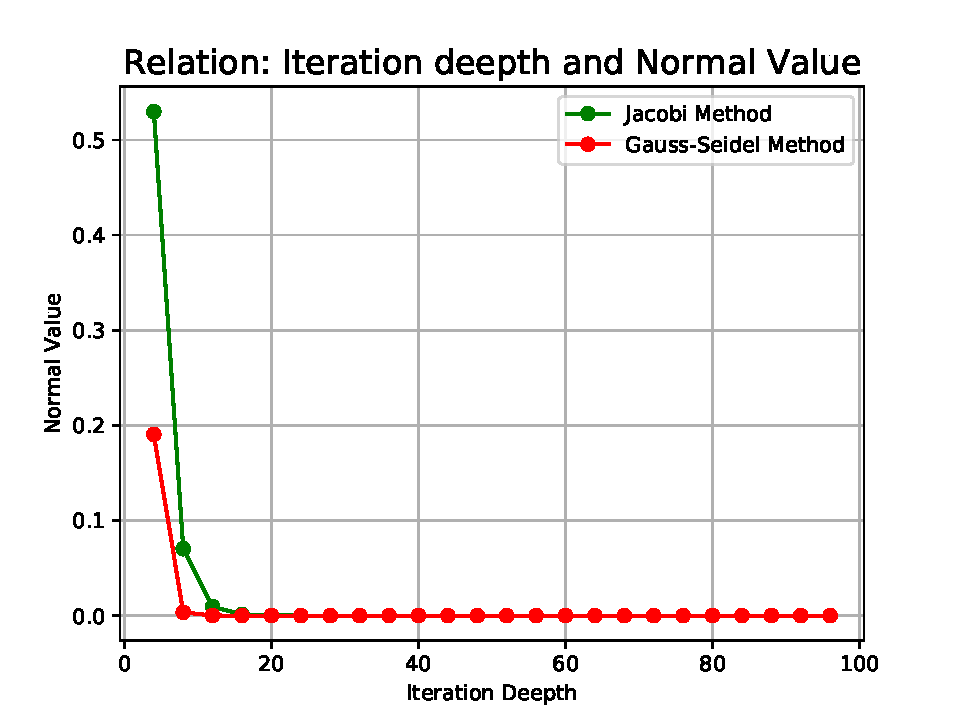
\includegraphics[width=0.7\textwidth]{../../img/04/compare.pdf}
    \caption{分组密码}
    \label{Fig:分组密码}
\end{figure}

\subsubsection{结果分析}
可以发现,在相同的迭代次数下,高斯-赛德尔方法的精度更高。

%%%%%%%%%%%%%%%%%%%%%%%%%%%%%%%%%%%%%%%%%%%%%%%%%%%%%%%%%%%%%%%%%%%%%%%%%%%%%%%%
%%%%%%%%%%%%%%%%%%%%%%%%%%%%%%%%%%% PROBLEM %%%%%%%%%%%%%%%%%%%%%%%%%%%%%%%%%%%%
%%%%%%%%%%%%%%%%%%%%%%%%%%%%%%%%%%%%%%%%%%%%%%%%%%%%%%%%%%%%%%%%%%%%%%%%%%%%%%%%

\subsection{第5题}
\begin{quote}
    {\kaishu
        用松弛法解
        \begin{equation}
            \left\{\begin{array}{r}{4 x_{1}-x_{2}=1} \\ {-x_{1}+4 x_{2}-x_{3}=4} \\ {-x_{2}+4 x_{3}=-3}\end{array}\right.
        \end{equation}
    分别取$w=1.03$,$w=1$,$w=1.1$。要求当$\left\|x^{(K)}-x^{(K-1)}\right\|<5 \times 10^{-6}$时迭代终止,并对每个$w$值确定迭代次数(初值$x^{(0)}=(0,0,0)^{\mathrm{T}}$)
    }
\end{quote}

程序代码参见\ref{4_5_Relaxation_Method.py}。

\subsubsection{运行结果}

\begin{figure}[H]   %H为当前位置,!htb为忽略美学标准,htbp为浮动图形
    \centering
    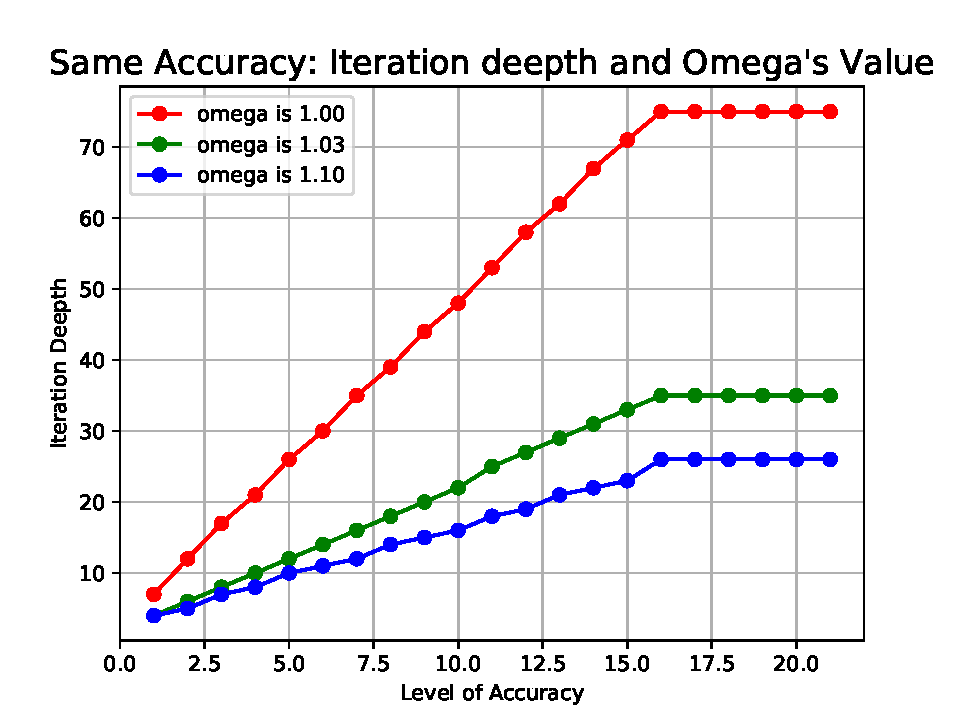
\includegraphics[width=0.7\textwidth]{../../img/04/relax.pdf}
    \caption{Relaxation}
    \label{Fig:relax}
\end{figure}

\subsubsection{结果分析}
本题代码行数比较多,而且涉及到了多个类的交互,所以对于参数的设计、传递,都有着巨大的考验,为了能够顺利构建出最终的图像,必须把class Matrix的对外行为设计得合乎规范,这样才能保证在调用矩阵的方法时毫无差错。可以从Code Analysis 1中看到,矩阵的所有方法,都没有改变该矩阵,换言之,这个类是不可更改的。这要求调用的时候,必须参考这一原则,写清楚赋值语句。而第二个类class Ma-trixIterMethod中,三个方法都列入了其中,虽然本题从实质上并没有调用雅可比方法,不过从先前的实验中可以看到,相同的精度下,它需要的迭代次数更多。

本段代码的更改经历了很长的时间,最终发现只有深刻理解才能写出程序。超松弛迭代法有着很深刻的数学经验在里面,而且在这里,超松弛迭代也经历了一个从一般分量形式到矩阵形式的转换。从时间统筹角度看,采用MATLAB进行编程会更加方便,也可以留出更多的时间来进行理论学习。


\section{实验体会}

从某种意义上讲,本次实验选错了语言,可能用基于矩阵的MATLAB会更加方便,而Python的numpy并不支持原生运算符,所以还是存在一定的局限性。

本试验报告的所有数据都经过MATLAB的验证,俱无问题。

如果有可能,在以后的实验报告中我将采用MATLAB进行编程。

\section{参考文献}

\printbibliography[heading=none]


\section{代码附录}
\label{附录}

\subsubsection{矩阵范数}
\lstinputlisting[
    style       =   Python,
    caption     =   {\bf 4\_1\_Normal\_Value.py},
    label       =   {4_1_Normal_Value.py}
]{../../src/4_解线性方程组的迭代法/4_1_Normal_Value.py}

\subsection{条件数}
\lstinputlisting[
    style       =   Python,
    caption     =   {\bf 4\_2\_Conditional\_Value.py},
    label       =   {4_2_Conditional_Value.py}
]{../../src/4_解线性方程组的迭代法/4_2_Conditional_Value.py}

\subsection{高斯-塞德尔迭代法}
\lstinputlisting[
    style       =   Python,
    caption     =   {\bf 4\_3\_Gauss–Seidel\_Iteration\_Method.py},
    label       =   {4_3_Gauss–Seidel_Iteration_Method.py}
]{../../src/4_解线性方程组的迭代法/4_3_Gauss–Seidel_Iteration_Method.py}

\subsection{作图}
\lstinputlisting[
    style       =   Python,
    caption     =   {\bf 4\_4\_Plot.py},
    label       =   {4_4_Plot.py}
]{../../src/4_解线性方程组的迭代法/4_4_Plot.py}

\subsection{松弛法}
\lstinputlisting[
    style       =   Python,
    caption     =   {\bf 4\_5\_Relaxation\_Method.py},
    label       =   {4_5_Relaxation_Method.py}
]{../../src/4_解线性方程组的迭代法/4_5_Relaxation_Method.py}

\end{document}
